\section{Multi-PE Platform}
\label{sec:multihost}


In this section we consider a platform with $N{>}1$ independently
schedulable PEs.  A direct extension of the dynamic programming approach in
the previous section would entail tracking the joint state of all task
executions on all PEs. The state space is thus combinatorial in $N$
(exponential with a straightforward representation), making the algorithm
no longer pseudo-polynomial time (if $N$ is considered part of the input).
Even for fixed $N{>}1$, its time and space requirements would likely be
prohibitive in practice.  Proposition~\ref{prop:np} establishes weak
NP-hardness for the one-PE case. Whether a stronger complexity result is
possible for the multi-PE case is an open question. Hereafter, we
present several heuristics, some of which build on the one-PE dynamic program.

\subsection{Heuristics}
\label{sec:multi-host:heuristics}

As in the one-PE case, we consider the
\dynamic heuristic (which is executed independently at each PE) and the
\random heuristic.  Section~\ref{sec:onehost:heuristics} describes eight
one-PE heuristics: nearsighted (\nearsighted) vs.  foresighted
(\foresighted), using one of four different criteria to select execution
modes (\errorlevel, \probsuccess, \ratio, \expectederror).  We extend these
heuristics to account for the simultaneous availability of all $N$ PEs at
time zero: given the $K{\geq}1$ possible execution modes for $T_1$, the
goal is to determine $n_1, n_2, \ldots, n_K$, where $n_j$ is the number of
PEs that will execute $T_1$ with mode $j$.  We initially set all $n_j$'s to
zero and compute their values greedily.  At each step, we
consider the option of incrementing one of the $n_j$'s (by one), leaving
all others at their current value.  Among these $K$ options, we pick the
one that leads to the best value of the scheduling criterion used by the
heuristic. This process is repeated until $\sum_{j=1}^{K} n_j = N$.
Hereafter we refer to these eight multi-PE heuristics as the ``greedy"
heuristics.

\subsection{Temporal Redundancy}

The design space for temporal redundancy is larger than in the one-PE case,
and we consider three options: 
\begin{compactitem}
	\item \textbf{Independent} (\independent) -- Use temporal redundancy 
	independently at each PE whenever it becomes idle due to 
	$T_M$ completing successfully.

	\item \textbf{Dependent} (\dependent) -- When $T_M$ completes successfully at a PE,
	  all PEs whose current executions cannot possibly achieve a lower error (due
	  to error levels achieved so far) abort their executions and apply
	  temporal redundancy.

	\item \textbf{Aggressive} (\aggressive) -- When $T_M$ completes successfully
	at a PE, all other PEs abort their
	executions and apply temporal redundancy.

\end{compactitem}


\subsection{Reactive Rescheduling}

With multiple PEs, there is an opportunity for
\emph{reactive rescheduling}: upon the completion 
of a task execution at a PE, other PEs can abort their ongoing task
executions and perform new scheduling decisions.  We consider three
options:

\begin{compactitem}
	\item \textbf{Off} (\off) -- No reactive rescheduling.

	\item \textbf{Variant} (\variant) -- Upon completion of task $T_i$ at
	PE $p$, if the ongoing application execution at PE $q{\neq}p$
	cannot achieve a lower overall error than the execution at PE
	$p$, then $q$ aborts its execution. An application execution
	is then restarted on PE $q$, but starting at task $T_{i+1}$. The
	input data provided to task $T_{i+1}$ is the output data from
	the execution of task $T_{i}$ at PE $p$.

	\item \textbf{Aggressive} (\aggressive) -- Upon completion of task $T_i$ at
	PE $p$, all other PEs abort their ongoing application executions
	and restart their executions at task $T_{i+1}$. The input data
	provided to task $T_{i+1}$ is the output data from the execution of
	task $T_{i}$ at PE $p$.
\end{compactitem}
\noindent

\subsection{Evaluation Methodology}

We define a scheduling strategy as a combination of \emph{design choices},
\strategy{A}{B}{C}, where A is the heuristic, B is the temporal redundancy
scheme, and C is the reactive rescheduling scheme.  Our goal is to
determine which design choices, and combinations thereof, lead to effective
scheduling strategies.  To this end, we perform one-to-one comparisons
between strategies that differ only in one particular design choice,
holding all other design choices fixed.

We evaluate these strategies in simulation for 470 different synthetic
application configurations and 25 random trials per configuration, for a
platform with $N{\in}\{2, 4, 8, 16\}$ PEs.  As in
Section~\ref{sec:onehost:heuristics} we use 2$\times$ and 5$\times$ $\efail$
multipliers.  With 5$\times$, there is a larger spread
between the high- and low-performing strategies (due to a larger penalty
for not meeting the deadline).  But the conclusions drawn from our results
and the ranking of the high-performing strategies when
considering $\efail$ multiplier values separately or combined are
unchanged.  Hereafter, we only discuss the combined results.  

As in Section~\ref{sec:onehost:heuristics}, we compare two strategies $X$ and
$Y$ using bootstrap confidence intervals of their relative differences in
mean error.  We say that $Y$ \emph{outperforms}, resp. \emph{is
outperformed} by, $X$ when the interval is strictly positive, resp.
negative.  When the interval contains zero, 
we say that the two strategies tie. To quantify the sensitivity of our
results to the (number of) samples, we performed 500 random split-half
analyses.  Overall, the top-performing strategy (see
Section~\ref{sec:multihost:regime}) is identical for 100\%, 86\%, 100\%,
and 100\% of the half-samples, for $N{=}2, 4, 8,$ and 16, respectively.

Regardless of $N,$ strategies that use \random are at best in the bottom 55\% of
strategies, and lead to mean error at least $3.52\times$ larger and up to $7.72\times$ larger than that of the
best-performing strategy.
We exclude \random from all results hereafter, considering thus
$8{+}1{=}9$ heuristics for a total of $9{\times}3{\times}3{=}81$
strategies.

\subsection{Design Choices for the Greedy Heuristics}

\noindent{\bf Is the multi-PE greedy extension useful?} -- Yes. We conduct
experiments in which each of the eight one-PE heuristics is used
independently at each PE. Each such heuristic, for any given temporal
redundancy and reactive rescheduling scheme, is outperformed by or ties
with its greedy counterpart.  Out of 72 one-to-one comparisons (eight
heuristics, three temporal redundancy schemes, three reactive rescheduling
schemes), the one-PE version is outperformed in 17, 26, 24, and 24 of them
for $N{=}2, 4, 8$, and 16, respectively, where all others are ties.  The
mean error improvement of the greedy version grows with $N$, from 3.6\% on
average for $N{=}2$ to 29.4\% on average for $N{=}16$. Expectedly,
considering all PEs jointly matters more as $N$ grows.  We consider only
the greedy heuristics hereafter.

\noindent{\bf Is foresighted scheduling worthwhile?} --
Yes. Out of 36 one-to-one comparisons (four scheduling criteria, three temporal redundancy schemes, three reactive rescheduling schemes),  \foresighted
outperforms \nearsighted in 27, 27, 27, and 21 of them for $N{=}2, 4,
8$, and 16, respectively, with \nearsighted leading to a mean error higher
by 67.2\% to 182.3\% on average, depending on
$N$.  In the remaining comparisons, \nearsighted outperforms \foresighted in 9, 3, 3, and 9 
cases, with mean error lower by 1.9\% to 14.4\% on average, and the two tie otherwise.  
Hereafter, we only consider \foresighted.

\noindent{\bf Which criteria should be used?} --
\probsuccess is ineffective. Despite being the second best criterion for one PE
(Section~\ref{sec:onehost:heuristics}), it is outperformed by
\expectederror for every temporal redundancy/reactive rescheduling scheme.
We surmise this is because, unlike the other criteria, it does not account for the magnitude
of the error. Hereafter, we no longer consider it. 
The relative effectiveness of the other criteria depends on $N$:
\begin{compactitem}
	\item $N{\leq}4$: \expectederror is best, then \ratio, then \errorlevel;
	\item $N{=}8$: \ratio is best, then \expectederror, then \errorlevel;
	\item $N{=}16$: \errorlevel is best, then \ratio, then \expectederror.
\end{compactitem}
\noindent
We find that \expectederror (the criterion most directly tied to the
objective, and the best one for the one-PE case) should be used when resources are scarce, 
but one should use simpler criteria when resources are plentiful and failures are
less of a concern. 
%Most likely why \probsuccess (which favors
%fast, high-error modes) gets worse and worse, while \errorlevel (which
%doesn't care about failures) becomes more competitive.

\noindent{\bf Which temporal redundancy option is best?} --
\dependent is best.  \dependent and \independent perform almost
identically.  Out of 36 one-to-one comparisons (three scheduling criteria,
three reactive rescheduling schemes, four $N$ values), they tie 31 times,
\dependent outperforming \independent with mean error lower by at most
0.01\% for the other 5 comparisons.  For each $N$ value, \dependent
outperforms \aggressive in three of the nine one-to-one comparisons,
\aggressive leading to mean error higher by 0.8\%, 3.0\%, 8.2\%, and 22.3\%
on average for $N=2, 4, 8,$ and 16, respectively.  \aggressive outperforms
\dependent for only one of the nine one-to-one comparisons for each $N$
value, with mean error at most 1.4\% lower.  Overall, \dependent is never
outperformed by \independent and outperforms \aggressive more often than it is
outperformed by it (and when outperformed by it, it is only marginally so).
This is because \aggressive can prematurely terminate executions that could
produce good results, and because \independent simply does not capitalize
on the work accomplished by other PEs.  Hereafter, we only consider
\dependent.

%All other pairs tied, especially for those using \aggressive reactive
%rescheduling, since then the completion of $T_M$ at any PE makes all other
%PEs abort, and the three temporal options behave identically. 

\noindent{\bf Should reactive rescheduling be used?} --
Yes, except perhaps for large $N$. For each of the three 
scheduling criteria,
\variant and \aggressive perform
nearly identically across all $N$ values (relative differences in mean error at most
0.7\%).  For $N{\leq}8$, \off is outperformed by the other two options. For
instance, \aggressive leads to mean error lower by 46.4\%, 67.7\%, and 66.8\%
on average for $N{=}2, 4$, and 8, respectively. For $N{=}16$, \off
is outperformed for two of the scheduling criteria (by 60.6\% on average). However,
for the \expectederror criterion, \variant and \aggressive lead to mean error higher than that of
\off by at least 103.5\%. While this may seem surprising, with
many PEs, there is a larger chance that a ``too risky" execution path is
``lucky" and completes a task relatively early. In this case, reactive
rescheduling will cause all PEs to embark on that same path, whereas \off
ends up being a better, more risk-averse option.  Overall, reactive
rescheduling is beneficial when resources are scarce, but it could be
detrimental as the number of PEs increases.  Hereafter, we only consider
\aggressive and \off.



\subsection{Design Choices for the \dynamic Heuristic}

\noindent{\bf Should reactive rescheduling be used?} --
Yes, with \aggressive. We note that \aggressive is only slightly better than
\variant: For each of the three temporal redundancy options and the four $N$
values, \aggressive is never outperformed by \variant, and leads to mean error
lower by at most 0.6\%. \off is always detrimental and never outperforms
\aggressive. Recall that, for the greedy heuristics, \off can be beneficial.
This is not the case here because \dynamic better takes into account the time
remaining until the deadline.  \aggressive's mean error is lower than
\off's by 56.1\%, 72.9\%, 60.4\%, and 29.4\% on average for $N{=}2, 4,
8$, and 16, respectively. The error reduction eventually decreases with $N$, which is
the same trend as for the greedy heuristics: as resources become more
plentiful, reactive rescheduling becomes less useful (but not detrimental
even at $N{=}16$). Hereafter, we only consider the \aggressive option.

\noindent{\bf Does the temporal redundancy option matter?} --
No. With \aggressive reactive rescheduling, all three temporal redundancy
options yield identical results. This is because \aggressive reactive rescheduling
essentially subsumes temporal redundancy. Hereafter, out of the nine possible
strategies that use \dynamic, we only consider 
\strategy{\dynamic}{\dependent}{\aggressive} (using the same
\dependent temporal redundancy option as for the greedy heuristics).

\subsection{Which Heuristic for Which Regime?}
\label{sec:multihost:regime}

The results in the two previous sections identify the scheduling strategy
design choices that are effective. Excluding the choices that are ineffective
leaves us with seven strategies.
For each $N$ value, we perform one-to-one comparisons
and remove any strategy that is outperformed by any other.
This process results in the same three non-dominated strategies for
all $N$ values:
\strategy{\dynamic}{\dependent}{\aggressive},
\strategy{\foresighted-\errorlevel}{\dependent}{\aggressive}, and
\strategy{\foresighted-\ratio}{\dependent}{\aggressive}.

These three strategies all employ the \dependent temporal redundancy
scheme and the \aggressive reactive rescheduling scheme, but use
three different heuristics. 
Fig.~\ref{fig:ranking} shows the average percentage degradation from best
mean error for the three heuristics.  For $N{\leq}4$,
\dynamic outperforms its competitors by a significant margin (by more than
81\% and 24\% for $N{=}2$ and 4, respectively). In contrast, \dynamic
loses by large margins for $N{\geq}8$. For $N{=}8$, \foresighted-\ratio is
the clear winner, with its competitors leading to mean error higher by more than 50\%.  
For $N{=}16$, \foresighted-\errorlevel is
the best heuristic, with \foresighted-\ratio a close second.

\begin{figure}
        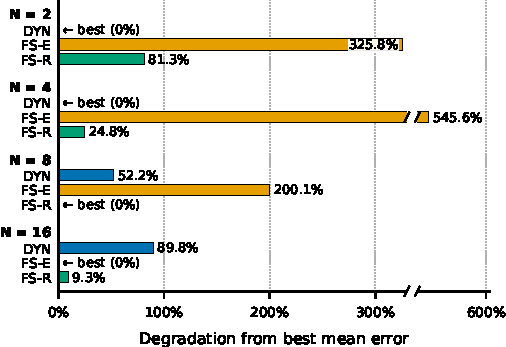
\includegraphics[width=\columnwidth]{./figures/multi_host_ranking.pdf}
	\caption{Average degradation from best mean error vs. $N$ for the heuristics used
	in the three non-dominated strategies.}
        \label{fig:ranking}
\end{figure}


We conclude that \dynamic is more competitive when resources are
scarce, i.e., when closer to the $N{=}1$ case.  As $N$ grows, it is
increasingly important to account for all PEs jointly, which \dynamic does
not do (as it is used independently at each PE).  Consequently, for larger
$N$, greedy heuristics, albeit less sophisticated in terms of local
scheduling decisions, become more competitive than and outperform \dynamic.


